\documentclass[tikz,border=6pt]{standalone}
\usepackage{xcolor}
\usepackage{newpxtext}
\usepackage{tikz}
\usetikzlibrary{shapes.geometric, arrows.meta, positioning, calc, fit, backgrounds, decorations.pathmorphing}

% Color Palette matching template.tex
\definecolor{SitePrimary}{RGB}{165, 124, 117}
\definecolor{DarkCharcoal}{HTML}{2B2B2B}
\definecolor{LightTaupe}{RGB}{245, 242, 240}
\definecolor{SubtleGray}{HTML}{F4F4F4}
\definecolor{BoxBorder}{HTML}{D0C9C5}
\definecolor{AccentRed}{HTML}{C62828}
\definecolor{AccentGreen}{HTML}{2E7D32}

\begin{document}
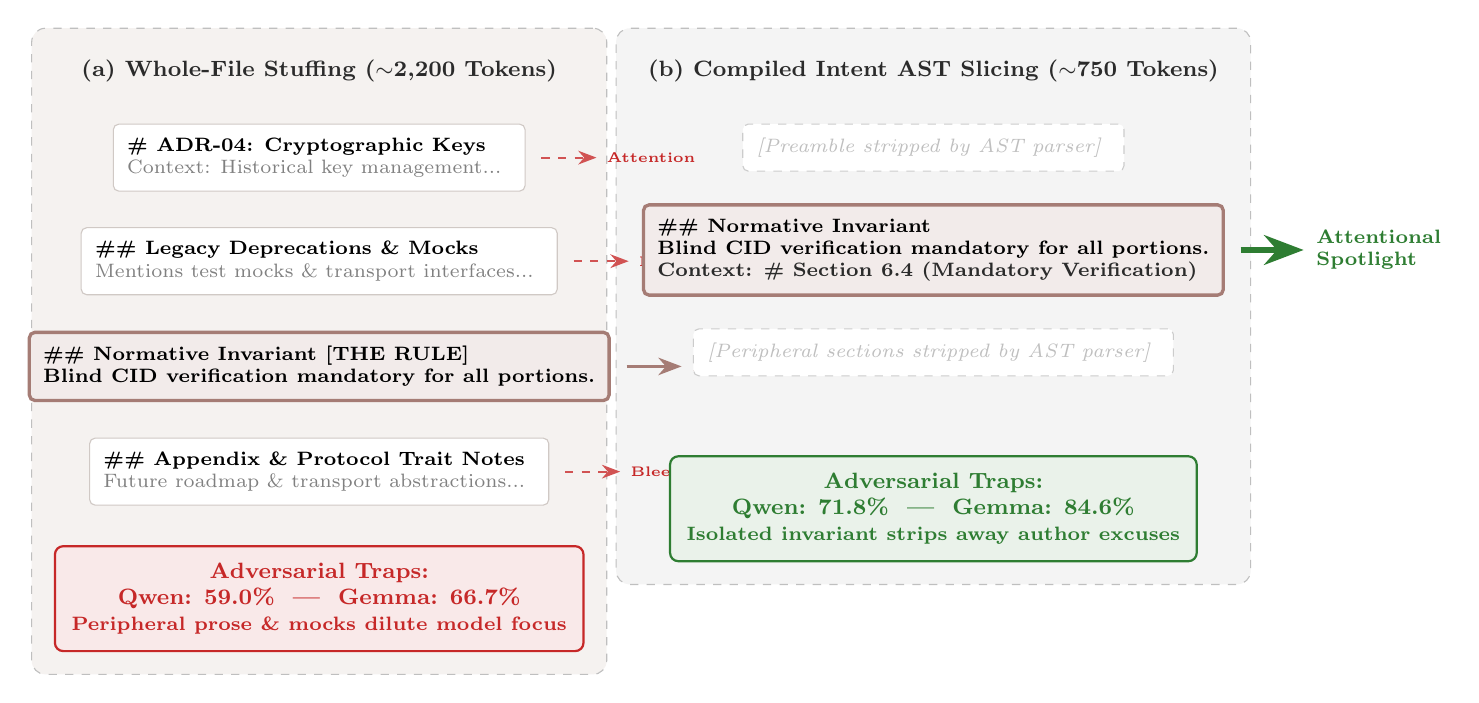
\begin{tikzpicture}[
    font=\small\color{DarkCharcoal},
    >=Stealth,
    node distance=0.45cm,
    docsection/.style={
        rectangle,
        draw=BoxBorder,
        fill=white,
        rounded corners=2pt,
        align=left,
        inner sep=5pt,
        minimum width=4.8cm,
        font=\scriptsize
    },
    needlesection/.style={
        rectangle,
        draw=SitePrimary,
        fill=SitePrimary!15!white,
        rounded corners=2pt,
        very thick,
        align=left,
        inner sep=5pt,
        minimum width=4.8cm,
        font=\scriptsize\bfseries
    },
    resultbadge/.style={
        rectangle,
        rounded corners=3pt,
        thick,
        align=center,
        inner sep=6pt,
        font=\footnotesize\bfseries,
        minimum width=4.8cm
    },
    subgraph/.style={
        draw=DarkCharcoal!30,
        fill=LightTaupe,
        rounded corners=5pt,
        dashed,
        inner sep=8pt
    }
]

    % ================= LEFT: Whole-File Stuffing =================
    \node[font=\footnotesize\bfseries\color{DarkCharcoal}] (title_a) at (0, 0) {(a) Whole-File Stuffing ($\sim$2,200 Tokens)};

    \node[docsection, below=0.4cm of title_a] (sec1) {
        \textbf{\# ADR-04: Cryptographic Keys}\\
        \color{gray}Context: Historical key management...
    };
    \node[docsection, below=of sec1] (sec2) {
        \textbf{\#\# Legacy Deprecations \& Mocks}\\
        \color{gray}Mentions test mocks \& transport interfaces...
    };
    \node[needlesection, below=of sec2] (sec3) {
        \textbf{\#\# Normative Invariant [THE RULE]}\\
        Blind CID verification mandatory for all portions.
    };
    \node[docsection, below=of sec3] (sec4) {
        \textbf{\#\# Appendix \& Protocol Trait Notes}\\
        \color{gray}Future roadmap \& transport abstractions...
    };

    % Attention bleed arrows
    \draw[->, thick, dashed, color=AccentRed!80] ($(sec1.east)+(0.2cm,0)$) -- ++(0.7cm, 0) node[right, font=\tiny\bfseries, text=AccentRed] {Attention};
    \draw[->, thick, dashed, color=AccentRed!80] ($(sec2.east)+(0.2cm,0)$) -- ++(0.7cm, 0) node[right, font=\tiny\bfseries, text=AccentRed] {Dilution};
    \draw[->, very thick, color=SitePrimary] ($(sec3.east)+(0.2cm,0)$) -- ++(0.7cm, 0) node[right, font=\tiny\bfseries, text=SitePrimary] {Needle};
    \draw[->, thick, dashed, color=AccentRed!80] ($(sec4.east)+(0.2cm,0)$) -- ++(0.7cm, 0) node[right, font=\tiny\bfseries, text=AccentRed] {Bleed};

    \node[resultbadge, draw=AccentRed, fill=AccentRed!10!white, text=AccentRed, below=0.5cm of sec4] (res_a) {
        Adversarial Traps:\\Qwen: 59.0\% ~|~ Gemma: 66.7\%\\{\scriptsize Peripheral prose \& mocks dilute model focus}
    };

    % Left Subgraph Background
    \begin{scope}[on background layer]
        \node[subgraph, fit=(title_a) (sec1) (sec4) (res_a)] (box_a) {};
    \end{scope}

    % ================= RIGHT: Compiled Intent AST Chunking =================
    \node[font=\footnotesize\bfseries\color{DarkCharcoal}] (title_b) at (7.8cm, 0) {(b) Compiled Intent AST Slicing ($\sim$750 Tokens)};

    \node[docsection, draw=gray!40, text=gray!50, dashed, below=0.4cm of title_b] (cut1) {
        \textit{[Preamble stripped by AST parser]}
    };
    
    \node[needlesection, draw=SitePrimary, fill=SitePrimary!15!white, below=0.4cm of cut1] (ast_chunk) {
        \textbf{\#\# Normative Invariant}\\
        Blind CID verification mandatory for all portions.\\
        {\scriptsize\color{DarkCharcoal}Context: \# Section 6.4 (Mandatory Verification)}
    };

    \node[docsection, draw=gray!40, text=gray!50, dashed, below=0.4cm of ast_chunk] (cut2) {
        \textit{[Peripheral sections stripped by AST parser]}
    };

    % Concentrated Attention Arrow
    \draw[->, line width=2.5pt, color=AccentGreen] ($(ast_chunk.east)+(0.2cm,0)$) -- ++(0.8cm, 0) 
        node[right, align=left, font=\scriptsize\bfseries, text=AccentGreen] {Attentional\\Spotlight};

    \node[resultbadge, draw=AccentGreen, fill=AccentGreen!10!white, text=AccentGreen, below=1.0cm of cut2] (res_b) {
        Adversarial Traps:\\Qwen: 71.8\% ~|~ Gemma: 84.6\%\\{\scriptsize Isolated invariant strips away author excuses}
    };

    % Right Subgraph Background
    \begin{scope}[on background layer]
        \node[subgraph, fit=(title_b) (cut1) (cut2) (res_b), fill=SubtleGray] (box_b) {};
    \end{scope}

\end{tikzpicture}
\end{document}
